\documentclass{standalone}
\usepackage{tikz}
\usetikzlibrary{patterns, positioning}
\usepackage[sfdefault]{ClearSans} %% option 'sfdefault' activates Clear Sans as the default text font
\usepackage[T1]{fontenc}

\begin{document}
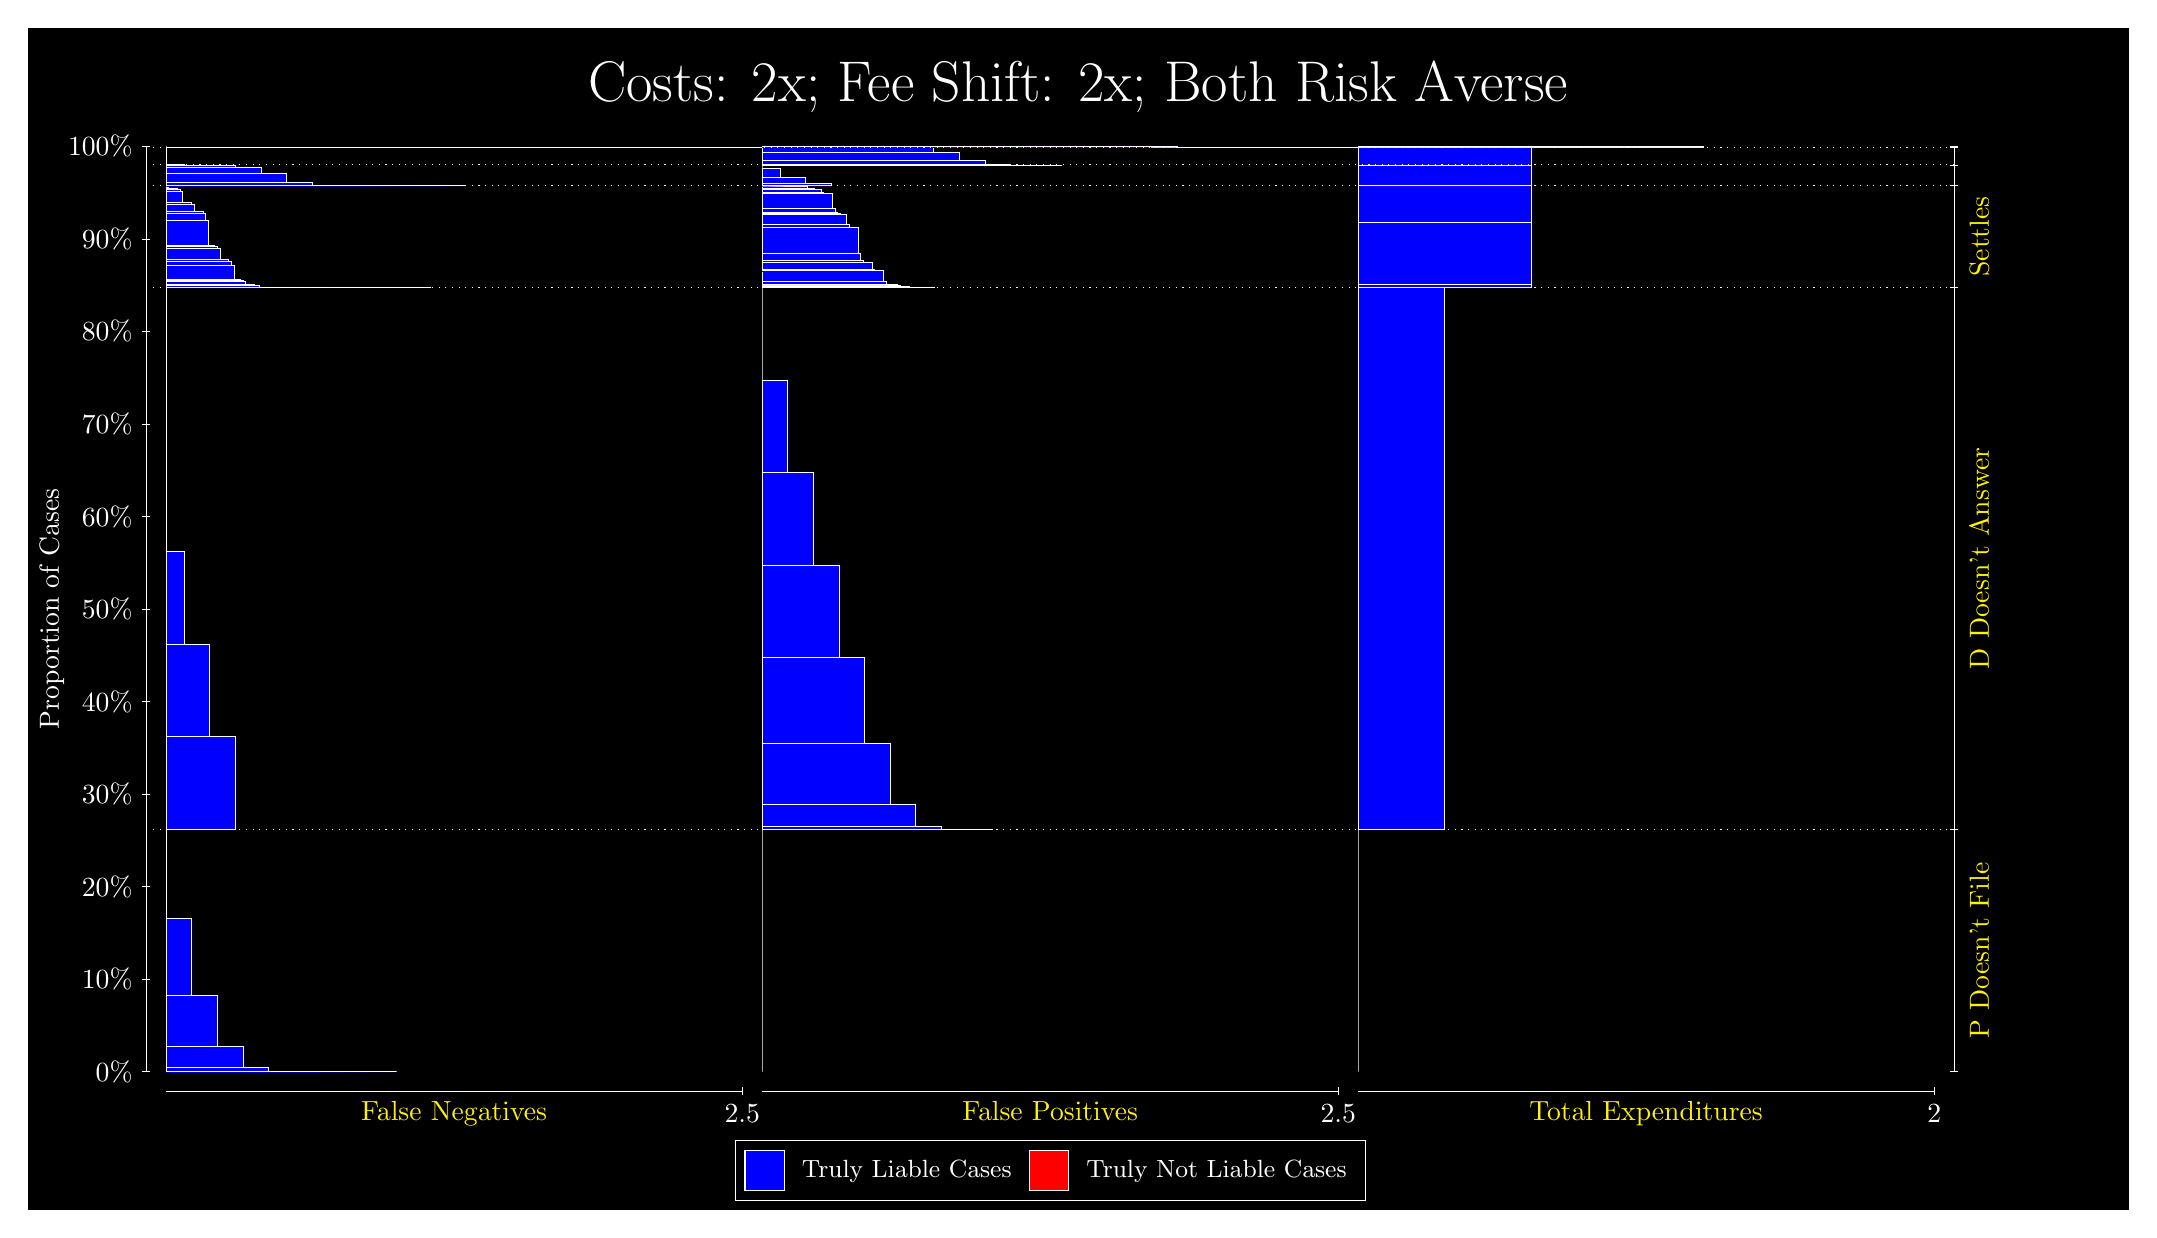
\begin{tikzpicture}
\draw[fill=black] (0,0) rectangle (26.667,15);
\draw[text=white] (0,13.5) rectangle (26.667,15) node[midway] {\huge Costs: 2x; Fee Shift: 2x; Both Risk Averse};
\draw[white, very thin] (1.5,1.75) -- (1.5,13.5);
\node[rotate=90, text=white, anchor=center] at (0.3, 7.625) {Proportion of Cases};
\draw[white, very thin] (1.45,1.75) -- (1.55,1.75);
\node[text=white, anchor=east] at (1.45, 1.75) {0\%};
\draw[white, very thin] (1.45,2.925) -- (1.55,2.925);
\node[text=white, anchor=east] at (1.45, 2.925) {10\%};
\draw[white, very thin] (1.45,4.1) -- (1.55,4.1);
\node[text=white, anchor=east] at (1.45, 4.1) {20\%};
\draw[white, very thin] (1.45,5.275) -- (1.55,5.275);
\node[text=white, anchor=east] at (1.45, 5.275) {30\%};
\draw[white, very thin] (1.45,6.45) -- (1.55,6.45);
\node[text=white, anchor=east] at (1.45, 6.45) {40\%};
\draw[white, very thin] (1.45,7.625) -- (1.55,7.625);
\node[text=white, anchor=east] at (1.45, 7.625) {50\%};
\draw[white, very thin] (1.45,8.8) -- (1.55,8.8);
\node[text=white, anchor=east] at (1.45, 8.8) {60\%};
\draw[white, very thin] (1.45,9.975) -- (1.55,9.975);
\node[text=white, anchor=east] at (1.45, 9.975) {70\%};
\draw[white, very thin] (1.45,11.15) -- (1.55,11.15);
\node[text=white, anchor=east] at (1.45, 11.15) {80\%};
\draw[white, very thin] (1.45,12.325) -- (1.55,12.325);
\node[text=white, anchor=east] at (1.45, 12.325) {90\%};
\draw[white, very thin] (1.45,13.5) -- (1.55,13.5);
\node[text=white, anchor=east] at (1.45, 13.5) {100\%};

\draw[white, very thin] (24.457,1.75) -- (24.457,13.5);
\draw[white, very thin] (24.407,1.75) -- (24.507,1.75);
\node[anchor=west] at (24.407, 1.75) {};
\draw[white, very thin] (24.407,4.8293) -- (24.507,4.8293);
\node[anchor=west] at (24.407, 4.8293) {};
\draw[white, very thin] (24.407,11.708) -- (24.507,11.708);
\node[anchor=west] at (24.407, 11.708) {};
\draw[white, very thin] (24.407,12.999) -- (24.507,12.999);
\node[anchor=west] at (24.407, 12.999) {};
\draw[white, very thin] (24.407,13.265) -- (24.507,13.265);
\node[anchor=west] at (24.407, 13.265) {};
\draw[white, very thin] (24.407,13.49) -- (24.507,13.49);
\node[anchor=west] at (24.407, 13.49) {};
\draw[white, very thin] (24.407,13.5) -- (24.507,13.5);
\node[anchor=west] at (24.407, 13.5) {};

\draw[white, very thin, fill=blue] (1.75,1.75) rectangle (4.6775,1.75);
\draw[white, very thin, fill=blue] (1.75,1.75) rectangle (4.3523,1.75);
\draw[white, very thin, fill=blue] (1.75,1.75) rectangle (4.027,1.75);
\draw[white, very thin, fill=blue] (1.75,1.75) rectangle (3.7017,1.7502);
\draw[white, very thin, fill=blue] (1.75,1.7502) rectangle (3.3764,1.755);
\draw[white, very thin, fill=blue] (1.75,1.755) rectangle (3.0511,1.8082);
\draw[white, very thin, fill=blue] (1.75,1.8082) rectangle (2.7258,2.0695);
\draw[white, very thin, fill=blue] (1.75,2.0695) rectangle (2.4006,2.7188);
\draw[white, very thin, fill=blue] (1.75,2.7188) rectangle (2.0753,3.7015);
\draw[white, very thin, fill=red] (1.75,3.7015) rectangle (1.75,3.7015);
\draw[white, very thin, fill=blue] (1.75,3.7015) rectangle (1.75,4.8293);
\draw[white, very thin, fill=blue] (1.75,4.8293) rectangle (2.6283,6.0044);
\draw[white, very thin, fill=blue] (1.75,6.0044) rectangle (2.303,7.1794);
\draw[white, very thin, fill=blue] (1.75,7.1794) rectangle (1.9777,8.3541);
\draw[white, very thin, fill=red] (1.75,8.3541) rectangle (1.75,8.3541);
\draw[white, very thin, fill=blue] (1.75,8.3541) rectangle (1.75,11.708);
\draw[white, very thin, fill=blue] (1.75,11.708) rectangle (5.1167,11.708);
\draw[white, very thin, fill=blue] (1.75,11.708) rectangle (4.9703,11.708);
\draw[white, very thin, fill=blue] (1.75,11.708) rectangle (4.8239,11.708);
\draw[white, very thin, fill=blue] (1.75,11.708) rectangle (4.7914,11.708);
\draw[white, very thin, fill=blue] (1.75,11.708) rectangle (4.6775,11.708);
\draw[white, very thin, fill=blue] (1.75,11.708) rectangle (4.645,11.708);
\draw[white, very thin, fill=blue] (1.75,11.708) rectangle (4.5312,11.708);
\draw[white, very thin, fill=blue] (1.75,11.708) rectangle (4.4986,11.708);
\draw[white, very thin, fill=blue] (1.75,11.708) rectangle (4.4661,11.708);
\draw[white, very thin, fill=blue] (1.75,11.708) rectangle (4.3848,11.708);
\draw[white, very thin, fill=blue] (1.75,11.708) rectangle (4.3523,11.708);
\draw[white, very thin, fill=blue] (1.75,11.708) rectangle (4.3197,11.708);
\draw[white, very thin, fill=blue] (1.75,11.708) rectangle (4.2384,11.708);
\draw[white, very thin, fill=blue] (1.75,11.708) rectangle (4.2059,11.708);
\draw[white, very thin, fill=blue] (1.75,11.708) rectangle (4.1734,11.708);
\draw[white, very thin, fill=blue] (1.75,11.708) rectangle (4.1408,11.708);
\draw[white, very thin, fill=blue] (1.75,11.708) rectangle (4.0595,11.708);
\draw[white, very thin, fill=blue] (1.75,11.708) rectangle (4.027,11.708);
\draw[white, very thin, fill=blue] (1.75,11.708) rectangle (3.9945,11.708);
\draw[white, very thin, fill=blue] (1.75,11.708) rectangle (3.9131,11.708);
\draw[white, very thin, fill=blue] (1.75,11.708) rectangle (3.8806,11.708);
\draw[white, very thin, fill=blue] (1.75,11.708) rectangle (3.8481,11.708);
\draw[white, very thin, fill=blue] (1.75,11.708) rectangle (3.8155,11.708);
\draw[white, very thin, fill=blue] (1.75,11.708) rectangle (3.7342,11.708);
\draw[white, very thin, fill=blue] (1.75,11.708) rectangle (3.7017,11.708);
\draw[white, very thin, fill=blue] (1.75,11.708) rectangle (3.6692,11.708);
\draw[white, very thin, fill=blue] (1.75,11.708) rectangle (3.5878,11.708);
\draw[white, very thin, fill=blue] (1.75,11.708) rectangle (3.5553,11.708);
\draw[white, very thin, fill=blue] (1.75,11.708) rectangle (3.5228,11.708);
\draw[white, very thin, fill=blue] (1.75,11.708) rectangle (3.4903,11.708);
\draw[white, very thin, fill=blue] (1.75,11.708) rectangle (3.4089,11.708);
\draw[white, very thin, fill=blue] (1.75,11.708) rectangle (3.3764,11.708);
\draw[white, very thin, fill=blue] (1.75,11.708) rectangle (3.3439,11.708);
\draw[white, very thin, fill=blue] (1.75,11.708) rectangle (3.2626,11.708);
\draw[white, very thin, fill=blue] (1.75,11.708) rectangle (3.23,11.709);
\draw[white, very thin, fill=blue] (1.75,11.709) rectangle (3.1975,11.709);
\draw[white, very thin, fill=blue] (1.75,11.709) rectangle (3.165,11.709);
\draw[white, very thin, fill=blue] (1.75,11.709) rectangle (3.0837,11.711);
\draw[white, very thin, fill=blue] (1.75,11.711) rectangle (3.0511,11.713);
\draw[white, very thin, fill=blue] (1.75,11.713) rectangle (3.0186,11.714);
\draw[white, very thin, fill=blue] (1.75,11.714) rectangle (2.9373,11.735);
\draw[white, very thin, fill=blue] (1.75,11.735) rectangle (2.9048,11.741);
\draw[white, very thin, fill=blue] (1.75,11.741) rectangle (2.8722,11.744);
\draw[white, very thin, fill=blue] (1.75,11.744) rectangle (2.8397,11.747);
\draw[white, very thin, fill=blue] (1.75,11.747) rectangle (2.7584,11.789);
\draw[white, very thin, fill=blue] (1.75,11.789) rectangle (2.7258,11.804);
\draw[white, very thin, fill=blue] (1.75,11.804) rectangle (2.6933,11.808);
\draw[white, very thin, fill=blue] (1.75,11.808) rectangle (2.612,11.988);
\draw[white, very thin, fill=blue] (1.75,11.988) rectangle (2.5795,12.043);
\draw[white, very thin, fill=blue] (1.75,12.043) rectangle (2.5469,12.06);
\draw[white, very thin, fill=blue] (1.75,12.06) rectangle (2.5144,12.066);
\draw[white, very thin, fill=blue] (1.75,12.066) rectangle (2.4331,12.203);
\draw[white, very thin, fill=blue] (1.75,12.203) rectangle (2.4006,12.236);
\draw[white, very thin, fill=blue] (1.75,12.236) rectangle (2.368,12.24);
\draw[white, very thin, fill=blue] (1.75,12.24) rectangle (2.2867,12.563);
\draw[white, very thin, fill=blue] (1.75,12.563) rectangle (2.2542,12.654);
\draw[white, very thin, fill=blue] (1.75,12.654) rectangle (2.2217,12.674);
\draw[white, very thin, fill=blue] (1.75,12.674) rectangle (2.1891,12.678);
\draw[white, very thin, fill=blue] (1.75,12.678) rectangle (2.1078,12.765);
\draw[white, very thin, fill=blue] (1.75,12.765) rectangle (2.0753,12.786);
\draw[white, very thin, fill=blue] (1.75,12.786) rectangle (2.0428,12.787);
\draw[white, very thin, fill=blue] (1.75,12.787) rectangle (1.9614,12.924);
\draw[white, very thin, fill=blue] (1.75,12.924) rectangle (1.9289,12.957);
\draw[white, very thin, fill=blue] (1.75,12.957) rectangle (1.8964,12.963);
\draw[white, very thin, fill=blue] (1.75,12.963) rectangle (1.7825,12.975);
\draw[white, very thin, fill=red] (1.75,12.975) rectangle (1.75,12.975);
\draw[white, very thin, fill=blue] (1.75,12.975) rectangle (1.75,12.999);
\draw[white, very thin, fill=blue] (1.75,12.999) rectangle (5.5558,12.999);
\draw[white, very thin, fill=blue] (1.75,12.999) rectangle (5.2305,12.999);
\draw[white, very thin, fill=blue] (1.75,12.999) rectangle (4.9052,12.999);
\draw[white, very thin, fill=blue] (1.75,12.999) rectangle (4.58,12.999);
\draw[white, very thin, fill=blue] (1.75,12.999) rectangle (4.2547,12.999);
\draw[white, very thin, fill=blue] (1.75,12.999) rectangle (3.9294,13.004);
\draw[white, very thin, fill=blue] (1.75,13.004) rectangle (3.6041,13.049);
\draw[white, very thin, fill=blue] (1.75,13.049) rectangle (3.2788,13.158);
\draw[white, very thin, fill=blue] (1.75,13.158) rectangle (2.9535,13.238);
\draw[white, very thin, fill=blue] (1.75,13.238) rectangle (2.6283,13.265);
\draw[white, very thin, fill=red] (1.75,13.265) rectangle (1.75,13.265);
\draw[white, very thin, fill=blue] (1.75,13.265) rectangle (2.6283,13.265);
\draw[white, very thin, fill=blue] (1.75,13.265) rectangle (2.303,13.265);
\draw[white, very thin, fill=blue] (1.75,13.265) rectangle (1.9777,13.266);
\draw[white, very thin, fill=red] (1.75,13.266) rectangle (1.75,13.266);
\draw[white, very thin, fill=blue] (1.75,13.266) rectangle (1.75,13.49);
\draw[white, very thin, fill=blue] (1.75,13.49) rectangle (9.9471,13.49);
\draw[white, very thin, fill=blue] (1.75,13.49) rectangle (9.6218,13.49);
\draw[white, very thin, fill=blue] (1.75,13.49) rectangle (9.2966,13.49);
\draw[white, very thin, fill=blue] (1.75,13.49) rectangle (8.9713,13.49);
\draw[white, very thin, fill=blue] (1.75,13.49) rectangle (8.9713,13.49);
\draw[white, very thin, fill=blue] (1.75,13.49) rectangle (8.646,13.49);
\draw[white, very thin, fill=blue] (1.75,13.49) rectangle (8.3207,13.49);
\draw[white, very thin, fill=blue] (1.75,13.49) rectangle (8.3207,13.49);
\draw[white, very thin, fill=blue] (1.75,13.49) rectangle (7.9954,13.49);
\draw[white, very thin, fill=blue] (1.75,13.49) rectangle (7.9954,13.49);
\draw[white, very thin, fill=blue] (1.75,13.49) rectangle (7.6702,13.491);
\draw[white, very thin, fill=blue] (1.75,13.491) rectangle (7.3449,13.492);
\draw[white, very thin, fill=blue] (1.75,13.492) rectangle (7.3449,13.493);
\draw[white, very thin, fill=blue] (1.75,13.493) rectangle (7.0196,13.494);
\draw[white, very thin, fill=blue] (1.75,13.494) rectangle (6.6943,13.494);
\draw[white, very thin, fill=blue] (1.75,13.494) rectangle (6.369,13.494);
\draw[white, very thin, fill=blue] (1.75,13.494) rectangle (6.369,13.494);
\draw[white, very thin, fill=blue] (1.75,13.494) rectangle (6.0437,13.494);
\draw[white, very thin, fill=blue] (1.75,13.494) rectangle (2.5957,13.494);
\draw[white, very thin, fill=blue] (1.75,13.494) rectangle (2.2705,13.494);
\draw[white, very thin, fill=blue] (1.75,13.494) rectangle (1.9452,13.494);
\draw[white, very thin, fill=blue] (1.75,13.494) rectangle (1.9452,13.494);
\draw[white, very thin, fill=red] (1.75,13.494) rectangle (1.75,13.494);
\draw[white, very thin, fill=blue] (1.75,13.494) rectangle (1.75,13.5);
\draw[white, very thin, fill=red] (9.3189,1.75) rectangle (9.3189,1.75);
\draw[white, very thin, fill=blue] (9.3189,1.75) rectangle (9.3189,4.8293);
\draw[white, very thin, fill=red] (9.3189,4.8293) rectangle (12.246,4.8293);
\draw[white, very thin, fill=blue] (9.3189,4.8293) rectangle (12.246,4.8294);
\draw[white, very thin, fill=blue] (9.3189,4.8294) rectangle (11.921,4.8306);
\draw[white, very thin, fill=blue] (9.3189,4.8306) rectangle (11.596,4.866);
\draw[white, very thin, fill=blue] (9.3189,4.866) rectangle (11.271,5.1479);
\draw[white, very thin, fill=blue] (9.3189,5.1479) rectangle (10.945,5.9236);
\draw[white, very thin, fill=blue] (9.3189,5.9236) rectangle (10.62,7.0157);
\draw[white, very thin, fill=blue] (9.3189,7.0157) rectangle (10.295,8.1832);
\draw[white, very thin, fill=blue] (9.3189,8.1832) rectangle (9.9694,9.3579);
\draw[white, very thin, fill=blue] (9.3189,9.3579) rectangle (9.6442,10.533);
\draw[white, very thin, fill=blue] (9.3189,10.533) rectangle (9.3189,11.708);
\draw[white, very thin, fill=red] (9.3189,11.708) rectangle (11.515,11.708);
\draw[white, very thin, fill=blue] (9.3189,11.708) rectangle (11.515,11.708);
\draw[white, very thin, fill=red] (9.3189,11.708) rectangle (11.368,11.708);
\draw[white, very thin, fill=blue] (9.3189,11.708) rectangle (11.368,11.709);
\draw[white, very thin, fill=red] (9.3189,11.709) rectangle (11.222,11.709);
\draw[white, very thin, fill=blue] (9.3189,11.709) rectangle (11.222,11.712);
\draw[white, very thin, fill=blue] (9.3189,11.712) rectangle (11.189,11.727);
\draw[white, very thin, fill=red] (9.3189,11.727) rectangle (11.075,11.727);
\draw[white, very thin, fill=blue] (9.3189,11.727) rectangle (11.075,11.732);
\draw[white, very thin, fill=blue] (9.3189,11.732) rectangle (11.043,11.744);
\draw[white, very thin, fill=red] (9.3189,11.744) rectangle (10.929,11.744);
\draw[white, very thin, fill=blue] (9.3189,11.744) rectangle (10.929,11.75);
\draw[white, very thin, fill=blue] (9.3189,11.75) rectangle (10.896,11.783);
\draw[white, very thin, fill=blue] (9.3189,11.783) rectangle (10.864,11.92);
\draw[white, very thin, fill=red] (9.3189,11.92) rectangle (10.783,11.92);
\draw[white, very thin, fill=blue] (9.3189,11.92) rectangle (10.783,11.921);
\draw[white, very thin, fill=blue] (9.3189,11.921) rectangle (10.75,11.942);
\draw[white, very thin, fill=blue] (9.3189,11.942) rectangle (10.718,12.029);
\draw[white, very thin, fill=red] (9.3189,12.029) rectangle (10.636,12.029);
\draw[white, very thin, fill=blue] (9.3189,12.029) rectangle (10.636,12.033);
\draw[white, very thin, fill=blue] (9.3189,12.033) rectangle (10.604,12.053);
\draw[white, very thin, fill=blue] (9.3189,12.053) rectangle (10.571,12.145);
\draw[white, very thin, fill=blue] (9.3189,12.145) rectangle (10.539,12.467);
\draw[white, very thin, fill=blue] (9.3189,12.467) rectangle (10.457,12.471);
\draw[white, very thin, fill=blue] (9.3189,12.471) rectangle (10.425,12.504);
\draw[white, very thin, fill=blue] (9.3189,12.504) rectangle (10.392,12.641);
\draw[white, very thin, fill=blue] (9.3189,12.641) rectangle (10.311,12.647);
\draw[white, very thin, fill=blue] (9.3189,12.647) rectangle (10.278,12.665);
\draw[white, very thin, fill=blue] (9.3189,12.665) rectangle (10.246,12.719);
\draw[white, very thin, fill=blue] (9.3189,12.719) rectangle (10.213,12.899);
\draw[white, very thin, fill=blue] (9.3189,12.899) rectangle (10.132,12.903);
\draw[white, very thin, fill=blue] (9.3189,12.903) rectangle (10.1,12.918);
\draw[white, very thin, fill=blue] (9.3189,12.918) rectangle (10.067,12.96);
\draw[white, very thin, fill=blue] (9.3189,12.96) rectangle (9.9857,12.963);
\draw[white, very thin, fill=blue] (9.3189,12.963) rectangle (9.9532,12.966);
\draw[white, very thin, fill=blue] (9.3189,12.966) rectangle (9.9206,12.972);
\draw[white, very thin, fill=blue] (9.3189,12.972) rectangle (9.8881,12.994);
\draw[white, very thin, fill=blue] (9.3189,12.994) rectangle (9.8068,12.994);
\draw[white, very thin, fill=blue] (9.3189,12.994) rectangle (9.7743,12.996);
\draw[white, very thin, fill=blue] (9.3189,12.996) rectangle (9.7417,12.998);
\draw[white, very thin, fill=blue] (9.3189,12.998) rectangle (9.6604,12.998);
\draw[white, very thin, fill=blue] (9.3189,12.998) rectangle (9.6279,12.999);
\draw[white, very thin, fill=blue] (9.3189,12.999) rectangle (9.5954,12.999);
\draw[white, very thin, fill=blue] (9.3189,12.999) rectangle (9.5628,12.999);
\draw[white, very thin, fill=blue] (9.3189,12.999) rectangle (9.4815,12.999);
\draw[white, very thin, fill=blue] (9.3189,12.999) rectangle (9.449,12.999);
\draw[white, very thin, fill=blue] (9.3189,12.999) rectangle (9.4165,12.999);
\draw[white, very thin, fill=blue] (9.3189,12.999) rectangle (9.3351,12.999);
\draw[white, very thin, fill=blue] (9.3189,12.999) rectangle (9.3189,12.999);
\draw[white, very thin, fill=red] (9.3189,12.999) rectangle (10.197,12.999);
\draw[white, very thin, fill=blue] (9.3189,12.999) rectangle (10.197,13.027);
\draw[white, very thin, fill=blue] (9.3189,13.027) rectangle (9.8718,13.106);
\draw[white, very thin, fill=blue] (9.3189,13.106) rectangle (9.5466,13.216);
\draw[white, very thin, fill=blue] (9.3189,13.216) rectangle (9.3189,13.265);
\draw[white, very thin, fill=red] (9.3189,13.265) rectangle (13.125,13.265);
\draw[white, very thin, fill=blue] (9.3189,13.265) rectangle (13.125,13.265);
\draw[white, very thin, fill=blue] (9.3189,13.265) rectangle (12.799,13.265);
\draw[white, very thin, fill=blue] (9.3189,13.265) rectangle (12.474,13.27);
\draw[white, very thin, fill=blue] (9.3189,13.27) rectangle (12.149,13.319);
\draw[white, very thin, fill=blue] (9.3189,13.319) rectangle (11.824,13.429);
\draw[white, very thin, fill=blue] (9.3189,13.429) rectangle (11.498,13.483);
\draw[white, very thin, fill=blue] (9.3189,13.483) rectangle (11.173,13.49);
\draw[white, very thin, fill=blue] (9.3189,13.49) rectangle (10.848,13.49);
\draw[white, very thin, fill=blue] (9.3189,13.49) rectangle (10.522,13.49);
\draw[white, very thin, fill=blue] (9.3189,13.49) rectangle (10.197,13.49);
\draw[white, very thin, fill=red] (9.3189,13.49) rectangle (17.516,13.49);
\draw[white, very thin, fill=blue] (9.3189,13.49) rectangle (17.516,13.49);
\draw[white, very thin, fill=red] (9.3189,13.49) rectangle (17.191,13.49);
\draw[white, very thin, fill=blue] (9.3189,13.49) rectangle (17.191,13.49);
\draw[white, very thin, fill=red] (9.3189,13.49) rectangle (16.865,13.49);
\draw[white, very thin, fill=blue] (9.3189,13.49) rectangle (16.865,13.49);
\draw[white, very thin, fill=red] (9.3189,13.49) rectangle (16.54,13.49);
\draw[white, very thin, fill=blue] (9.3189,13.49) rectangle (16.54,13.49);
\draw[white, very thin, fill=red] (9.3189,13.49) rectangle (16.215,13.49);
\draw[white, very thin, fill=blue] (9.3189,13.49) rectangle (16.215,13.49);
\draw[white, very thin, fill=red] (9.3189,13.49) rectangle (15.89,13.49);
\draw[white, very thin, fill=blue] (9.3189,13.49) rectangle (15.89,13.49);
\draw[white, very thin, fill=blue] (9.3189,13.49) rectangle (15.89,13.49);
\draw[white, very thin, fill=red] (9.3189,13.49) rectangle (15.564,13.49);
\draw[white, very thin, fill=blue] (9.3189,13.49) rectangle (15.564,13.49);
\draw[white, very thin, fill=blue] (9.3189,13.49) rectangle (15.564,13.49);
\draw[white, very thin, fill=red] (9.3189,13.49) rectangle (15.239,13.49);
\draw[white, very thin, fill=blue] (9.3189,13.49) rectangle (15.239,13.491);
\draw[white, very thin, fill=blue] (9.3189,13.491) rectangle (15.239,13.492);
\draw[white, very thin, fill=blue] (9.3189,13.492) rectangle (14.914,13.493);
\draw[white, very thin, fill=red] (9.3189,13.493) rectangle (14.914,13.493);
\draw[white, very thin, fill=blue] (9.3189,13.493) rectangle (14.914,13.493);
\draw[white, very thin, fill=blue] (9.3189,13.493) rectangle (14.914,13.494);
\draw[white, very thin, fill=blue] (9.3189,13.494) rectangle (14.588,13.495);
\draw[white, very thin, fill=blue] (9.3189,13.495) rectangle (14.588,13.495);
\draw[white, very thin, fill=blue] (9.3189,13.495) rectangle (14.588,13.495);
\draw[white, very thin, fill=blue] (9.3189,13.495) rectangle (14.263,13.496);
\draw[white, very thin, fill=blue] (9.3189,13.496) rectangle (14.263,13.496);
\draw[white, very thin, fill=blue] (9.3189,13.496) rectangle (13.938,13.496);
\draw[white, very thin, fill=blue] (9.3189,13.496) rectangle (13.938,13.496);
\draw[white, very thin, fill=blue] (9.3189,13.496) rectangle (13.938,13.496);
\draw[white, very thin, fill=blue] (9.3189,13.496) rectangle (13.613,13.496);
\draw[white, very thin, fill=blue] (9.3189,13.496) rectangle (13.613,13.496);
\draw[white, very thin, fill=blue] (9.3189,13.496) rectangle (13.613,13.496);
\draw[white, very thin, fill=blue] (9.3189,13.496) rectangle (13.287,13.496);
\draw[white, very thin, fill=blue] (9.3189,13.496) rectangle (13.287,13.496);
\draw[white, very thin, fill=blue] (9.3189,13.496) rectangle (13.287,13.496);
\draw[white, very thin, fill=blue] (9.3189,13.496) rectangle (12.962,13.496);
\draw[white, very thin, fill=blue] (9.3189,13.496) rectangle (12.637,13.496);
\draw[white, very thin, fill=blue] (9.3189,13.496) rectangle (12.311,13.496);
\draw[white, very thin, fill=blue] (9.3189,13.496) rectangle (11.986,13.496);
\draw[white, very thin, fill=red] (9.3189,13.496) rectangle (9.3189,13.496);
\draw[white, very thin, fill=blue] (9.3189,13.496) rectangle (9.3189,13.5);
\draw[white, very thin, fill=red] (16.888,1.75) rectangle (16.888,1.75);
\draw[white, very thin, fill=blue] (16.888,1.75) rectangle (16.888,4.8293);
\draw[white, very thin, fill=red] (16.888,4.8293) rectangle (17.986,4.8293);
\draw[white, very thin, fill=blue] (16.888,4.8293) rectangle (17.986,11.708);
\draw[white, very thin, fill=red] (16.888,11.708) rectangle (19.083,11.708);
\draw[white, very thin, fill=blue] (16.888,11.708) rectangle (19.083,11.754);
\draw[white, very thin, fill=red] (16.888,11.754) rectangle (19.083,11.754);
\draw[white, very thin, fill=blue] (16.888,11.754) rectangle (19.083,12.53);
\draw[white, very thin, fill=red] (16.888,12.53) rectangle (19.083,12.53);
\draw[white, very thin, fill=blue] (16.888,12.53) rectangle (19.083,12.999);
\draw[white, very thin, fill=red] (16.888,12.999) rectangle (19.083,12.999);
\draw[white, very thin, fill=blue] (16.888,12.999) rectangle (19.083,13.265);
\draw[white, very thin, fill=red] (16.888,13.265) rectangle (19.083,13.265);
\draw[white, very thin, fill=blue] (16.888,13.265) rectangle (19.083,13.49);
\draw[white, very thin, fill=red] (16.888,13.49) rectangle (21.279,13.49);
\draw[white, very thin, fill=blue] (16.888,13.49) rectangle (21.279,13.492);
\draw[white, very thin, fill=red] (16.888,13.492) rectangle (21.279,13.492);
\draw[white, very thin, fill=blue] (16.888,13.492) rectangle (21.279,13.495);
\draw[white, very thin, fill=red] (16.888,13.495) rectangle (21.279,13.495);
\draw[white, very thin, fill=blue] (16.888,13.495) rectangle (21.279,13.5);
\draw[white, dotted] (1.5,4.8293) -- (24.457,4.8293);
\draw[white, dotted] (1.5,11.708) -- (24.457,11.708);
\draw[white, dotted] (1.5,12.999) -- (24.457,12.999);
\draw[white, dotted] (1.5,13.265) -- (24.457,13.265);
\draw[white, dotted] (1.5,13.49) -- (24.457,13.49);
\draw[white, very thin] (1.75,1.5) -- (9.0689,1.5);
\node[text=yellow, anchor=north] at (5.4094, 1.5) {False Negatives};
\draw[white, very thin] (9.0689,1.45) -- (9.0689,1.55);
\node[text=white, anchor=north] at (9.0689, 1.45) {2.5};

\draw[white, very thin] (9.3189,1.5) -- (16.638,1.5);
\node[text=yellow, anchor=north] at (12.978, 1.5) {False Positives};
\draw[white, very thin] (16.638,1.45) -- (16.638,1.55);
\node[text=white, anchor=north] at (16.638, 1.45) {2.5};

\draw[white, very thin] (16.888,1.5) -- (24.207,1.5);
\node[text=yellow, anchor=north] at (20.547, 1.5) {Total Expenditures};
\draw[white, very thin] (24.207,1.45) -- (24.207,1.55);
\node[text=white, anchor=north] at (24.207, 1.45) {2};

\node[text=yellow, centered, rotate=90] at (24.777, 3.2897) {P Doesn't File};
\node[text=yellow, centered, rotate=90] at (24.777, 8.2686) {D Doesn't Answer};
\node[text=yellow, centered, rotate=90] at (24.777, 12.354) {Settles};




\draw (12.978300999999998,1.5) node[draw=none] (baseCoordinate) {};
\begin{scope}[align=center]
        \matrix[scale=0.5, draw=white, below=0.5cm of baseCoordinate, nodes={draw}, column sep=0.1cm]{
            \node[rectangle, draw, minimum width=0.5cm, minimum height=0.5cm, fill=blue] {}; &
            \node[draw=none, font=\small, text=white] (B) {Truly Liable Cases}; &
            \node[rectangle, draw, minimum width=0.5cm, minimum height=0.5cm, fill=red] {}; &
            \node[draw=none, font=\small, text=white] (B) {Truly Not Liable Cases}; \\
            };
\end{scope}

\end{tikzpicture}
\end{document}